\documentclass[twocolumn]{article}
\usepackage[utf8]{inputenc}
\usepackage{amsmath}
\usepackage{graphicx}
\usepackage{sectsty}
\usepackage{lipsum,multicol}

\allsectionsfont{\centering}
\font\myfont=cmr12 at 30pt
\title{\vspace{-2cm} \textbf{{\myfont Design and Analysis of Algorithms}} \\
\\Group-2
}


\author{Nidhi kamewar   \hspace{10ex}Rishi Mukesh Gupta \hspace{6ex}   Pechetti Venkata Karthik\\    
\hspace{4ex}  IIT2019189     \hspace{14ex}           IIT2019190       \hspace{18ex}           IIT2019191   \hspace{9ex}  
   


}



\begin{document}

\maketitle
\noindent
\textbf{
Abstract:Given weights and values of n items we have to design an algorithm to find out the maximum value subset of the values of final items which must be included in the knapsack such that the total value of the weight of the final items included in the knapsack should be less than or equal to  the given capacity of the knapsack}

\section*{I.INTRODUCTION}

In this problem,we have to maximise the value of the items included in the knapsack such that the weight of the items included does not exceed the given weight .\\
\\
As the given problem has Overlapping subproblems of recalculating the total value sum of the items included in the knapsack for a given limit of the knapsack and Optimal substructure property i.e the given problem can be solved by  solving the subproblems of the problem
\\
\\
Hence We can solve the given problem using Dynamic programming.
\\
\noindent\\
This report further contains -\\
\\
II. Algorithm Design \\
III. Algorithm Analysis\\
IV. Experimental Study\\
V. Conclusion\\
\\
\\
\\
\section*{II.ALGORITHM DESIGN
}

\centerline{\textbf{Algorithm-1}}\\
\noindent\\
1.We have to check for all possible valid subsets of the given set of values and respective weights 
\\
\noindent\\
2.There are two possible cases for every item either to be included or not to be included in the subset .\\
\noindent\\
3.By considering both of the cases we choose the one which gives us the maximum value of the items  for a given capacity of the knapsack.\\
\noindent\\
4.The function recursively calls itself to find the maximum value of the items excluding the current item and including the current item.\\
\noindent\\
5.If the weight of the current item is greater than the given capacity of the knapsack then we remove that item from the knapsack then we call the function for the remaining elements . \\

\centerline{\textbf{Algorithm-2}}\\
\\
\noindent\\
As the first algorithm is not very efficient as it recalculate same result we can remove the work of calculating the same result again by storing the value of the subproblems\\
\\
So we designed an algorithm  based on dynamic programming Tabular(Bottom-Up) Approach
\noindent\\
we reach our solution by considering all the subsolutions and storing the solutions to the subproblems in a lookup table which are filled iteratively until we reach the solution to the given problem  \\
\noindent\\
1.First, the array of values of the given items and weights of respective items are passed to the function \\
\noindent\\
2.we start at the initial condition of 0 weight limit which implies that the bag cannot be filled and so we fill the lookup table dp[][0] row to all 0’s and we fill the values of dp[0][] row to 0’s as there will be no  items included in the knapsack if there are no items given.\\
\noindent\\
3.The function iteratively fils the values of every cell of the lookup table,If the weight of the item is greater than the current knapsack limit the we cannot add the item into the knapsack so we leave the item i.e, we store the value of dp[i-1][j] in the cell dp[i][j].\\
\noindent\\
4.If the weight of the item is less than the current knapsack limit then we fill the cell with the maximum of  values attained by including the item in the knapsack(dp[i-1][j-wt[i-1]]+val[i-1]) and attained by not including the item in the knapsack (dp[i-1][j])\\
\noindent\\
5.Finally we return the value of dp[n][cap] which is the maximum value of the items which can be included in the knapsack.\\
\noindent\\
For Example:-\\
\\
Consider the following\\
\\
Values  Weights\\
3\space \space \space \space \space \space \space \space 	6\\
9\space \space \space \space \space \space \space \space4\\
2\space \space \space \space \space \space \space \space6\\
1\space \space \space \space \space \space \space \space1\\
6\space \space \space \space \space \space \space \space4	\\



\vfill\eject
\\
\\
Lookup table:\\





\begin{center}
	\begin{tabular}{ |c | c | c | c | c | c | c | c | c| }
	\hline
	  &0&1&2&3&4&5&6&7\\
	 \hline
	0&0&0&0&0&0&0&0&0\\
	\hline
	1&0&0&0&0&0&0&3&3\\
\hline
	2&0&0&0&0&9&9&9&9\\
\hline
	3&0&0&0&0&9&9&9&9\\
\hline
	4&0&1&1&1&9&10&10&10\\
\hline
	5&0&1&1&1&9&10&10&10\\
	\hline
	\end{tabular}
\end{center}



\noindent\\
By maintaining the lookup table we removed the task of recalculating the overlapping subproblems.\\
\noindent
For example in the above problem we the value of dp[1][3] is not recalculated but instead stored at the first calculation and stored in the lookup table and is directly used in other subproblem .\\
\\
\noindent\\
The algorithm builds the above lookup table iteratively till the last cell (dp[5][7]) which is the solution to our problem and finally returns the value present in the last cell.

\section*{PSEUDO CODE
}

\centerline{\textbf{Algorithm-1}}\\
\vspace{7px}
\hline
\vspace{10px}
\nointend\\
\textbf{function}  Solveknapsack( )\\
\\
   \noindent    \textbf{\qquad if}\: \:W==0 \:or\: n==0\:
	\textbf{then} \\
         \textbf{return }  0;\\
         \\
         \textbf{\qquad else if} wt[n-1]\textgreater \ Totalweight\\
            \textbf{return }  solveknapsack(val,wt,W,n-1)\\
            \\
    \textbf{\qquad else}\\
         \textbf{return } max\\(solveknapsack(val,wt,W,n-1),solveknapsack(val,wt,W-wt[n-1],n-1
+val[n-1]))\\
 \textbf{\qquad end if}
\\
\hline
\vfill\eject
\centerline{\textbf{Algorithm-2}}\\
\vspace{7px}
\hline
\vspace{10px}
\noindent  \\
\textbf{function}  Solveknapsack( )\\
\\
   \noindent    \textbf{\qquad if}\: \:i==0 \:or\:j==0\:
	\textbf{then} \\
         dp[i][j]← 0\\
\noindent  
         \\
         \textbf{\qquad else if} wt[i-1]\textgreater \ j
 \noindent     \\     
           dp[i][j]←dp[i-1][j];\\
            \\
            \noindent  
    \textbf{\qquad else}\\
        dp[i][j]← max(dp[i-1][j],dp[i-1][j-wt[i-1]]+val[i-1])
+val[n-1]))\\
 \textbf{\qquad end if}

 \vspace{10px}
 \hline
\section*{III.ALGORITHM ANALYSIS}
\centerline{\textbf{Algorithm-1}}\\
\\
\textbf{Time complexity}\\
\\
The algorithm -1 computes every possible subset to find the solution to the main problem hence it take $O(2^n)$ time as the possible cases for an item is either to be include or not be included \\
\\
\textbf{Space complexity}\\
\\
The algorithm uses O(1) auxiliary space as no extra data structures are required\\

\centerline{\textbf{Algorithm-2}}\\
\\

\textbf{Time complexity}\\
\\
The algorithm-2 does not compute the solutions to overlapping subproblems instead looks for them in the lookup table which stores the values of subproblems which occurred before.
\\
The algorithm stores the solutions  of every subproblem by bottom up approach by iterating through all possible subproblems i.e,the time complexity of the algorithm would be $O(n*cap)$.\\
\\
\vfill\eject
\textbf{Space complexity}\\
\\
The algorithm uses $O(n*cap)$ auxiliary space for the lookup table .\\


\section*{IV.EXPERIMENTAL STUDY
}
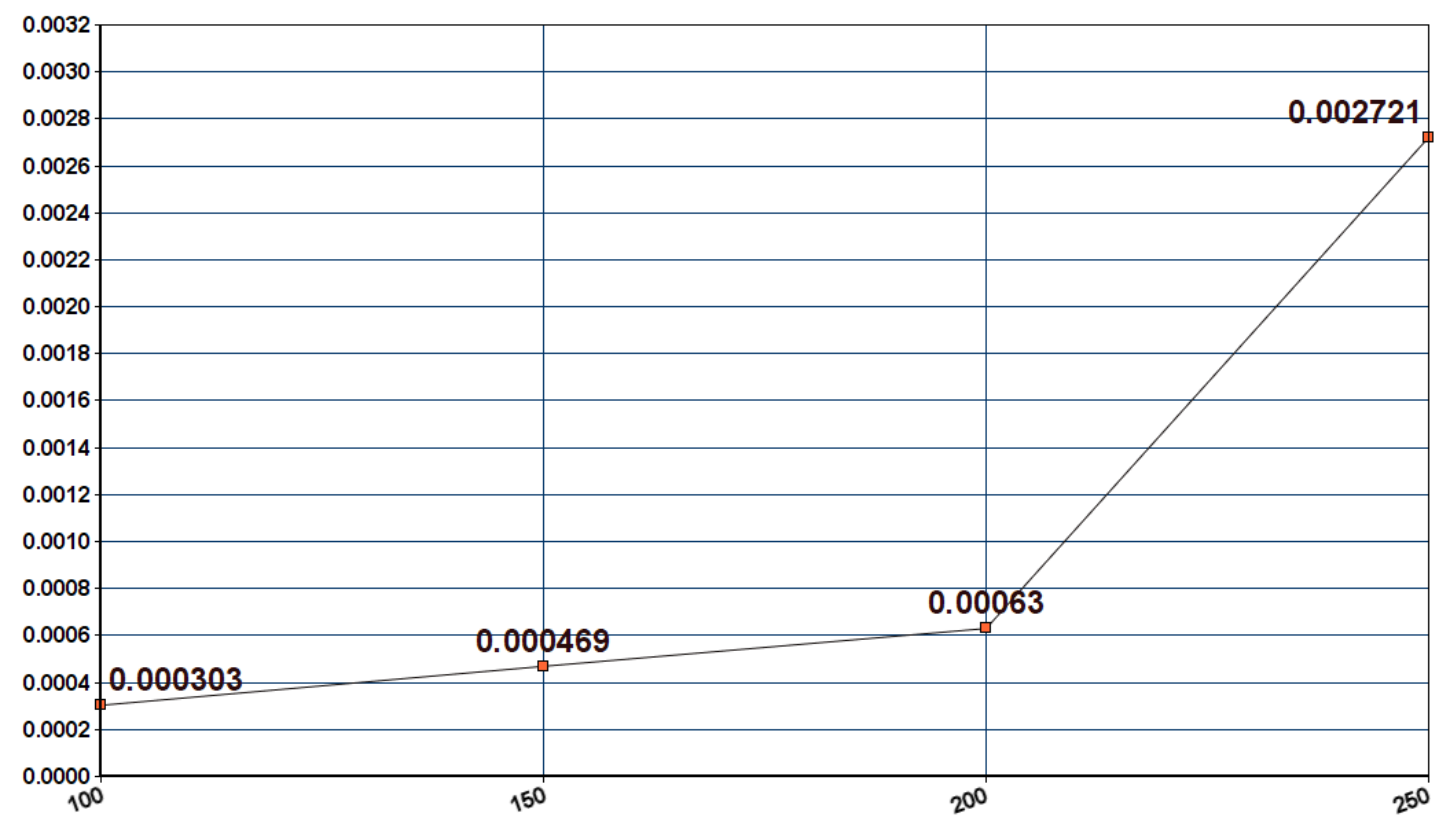
\includegraphics[width=.45\textwidth]{expo1.png}
\\
\centerline{Fig-1}\\
\begin{center}
	\begin{tabular}{ |c | c | }
	\hline
	
n(number of items)
X-axis
&
Time
Y-axis




 \\
	 \hline

100&
0.001525

\\
	\hline


150

&
0.009756

\\
\hline

200&
0.018425

\\
\hline

250&
0.056188

\\
\hline
	\end{tabular}
\end{center}
\\
\\
From the plotted graph (Fig-1) of test cases  we can see the time complexity of the algorithm-1 to be $O(2^n)$ by asymptotic analysis i.e,the time complexity is exponential 
\\
\\
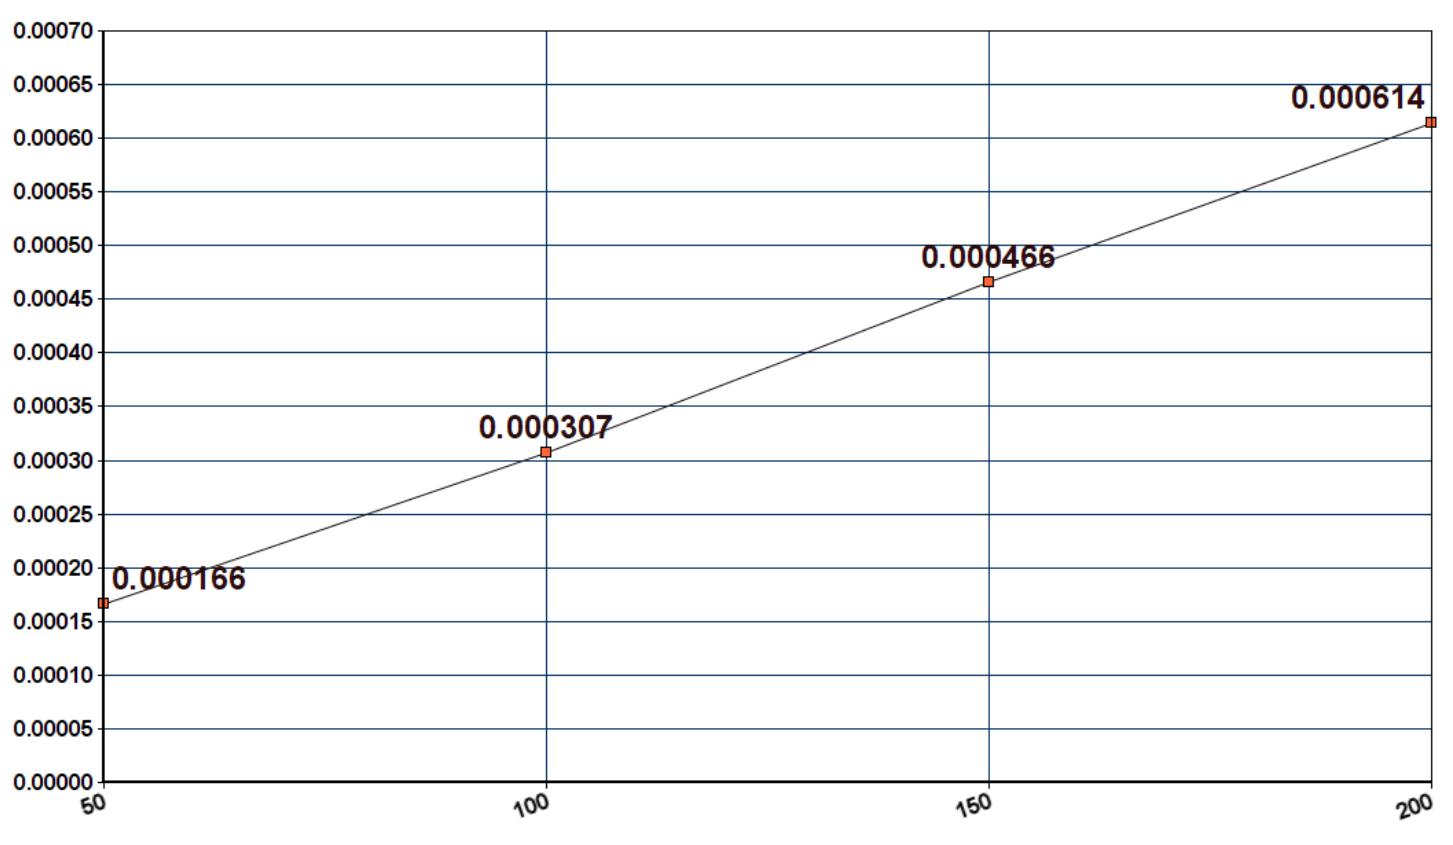
\includegraphics[width=.45\textwidth]{line2.png}
\centerline{Fig-2}
\begin{center}
	\begin{tabular}{ |c | c | c | }
	\hline
	
n(number of items)
X-axis
&
capacity&
Time
Y-axis




 \\
	 \hline


50&
950&
0.000166



\\
	\hline



100&
950&
0.000307



\\
\hline


150&
950&
0.000466


\\
\hline


200&
950&
0.000614



\\
\hline
	\end{tabular}
\end{center}
\\
Algorithm-2 is a more efficient algorithm as it uses dynamic programming to avoid recalculating the solutions to the overlapping subproblem wheares  the algorithm-1 uses exhaustive search by which arrives at the solution by generating all possible subsets .

From the plotted graph(Fig-2) we can see a linear growth of the graph when the capacity of the knapsack is constant as time complexity of algorithm is O(n*capacity)
 \vspace{10px}.
\\
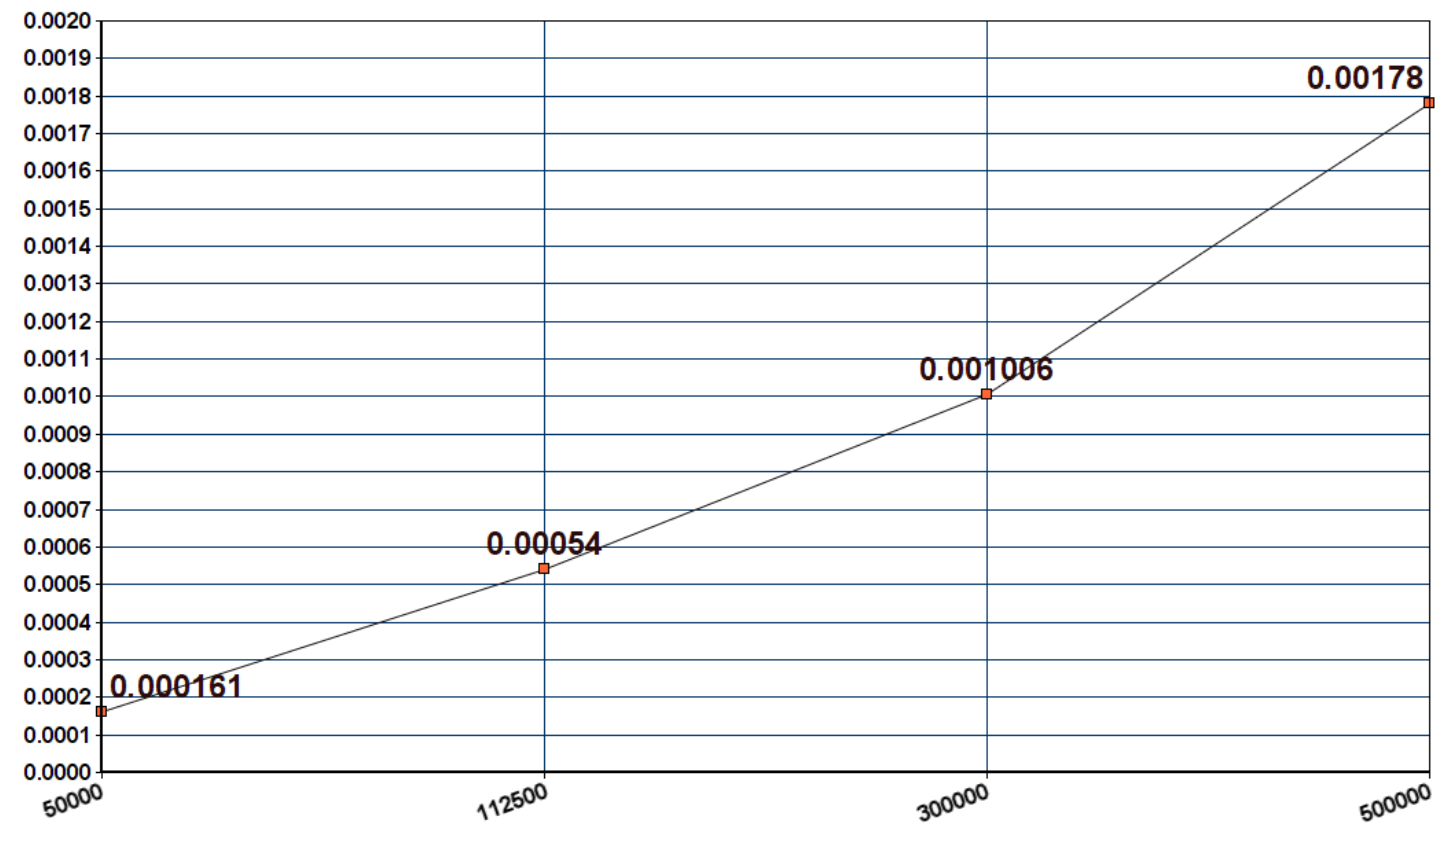
\includegraphics[width=.45\textwidth]{para3.png}
\centerline{Fig-3}\\
\begin{center}
	\begin{tabular}{ |c | c | c | }
	\hline
	
n(number of items)
X-axis
&
capacity&
Time
Y-axis







\\
	\hline



100&
950&
0.000307



\\
\hline


150&
950&
0.000466


\\
\hline


200&
950&
0.000614

 \\
	 \hline


250&
2000&
0.001780




\\
\hline
	\end{tabular}
\end{center}



From the plotted graph (Fig-3) where capacity is not constant we can see the time complexity of the graph to  be $O(n*capacity)$

\section*{V.CONCLUSION
}
From the experimental study we concluded that the time complexity  of the algorithm-2 $(O(n*capacity)) $is better than the first one $(O(2^n))$ which can be observed from the study of graphs of algorithm-1  and algorithm-2

\section*{REFERENCES    
}


  \phantom{x}\hspace{3ex}   1. https://www.geeksforgeeks.org
      
   \phantom{x}\hspace{0.97ex}   2. Introduction to Algorithms (CLRS)

\end{document}